\documentclass[11pt]{article}
\usepackage[T1]{fontenc}
\usepackage[utf8]{inputenc}
\usepackage{graphicx}
\usepackage{minitoc}
\usepackage[french]{babel}
\usepackage[right=2.5cm, bottom=2.5cm,top=2.5cm, left=2.5cm]{geometry}
\title{\vspace{\fill} Interface et Multimédia \\ ~\textbf{IFT-215} \\~\\ Travail Pratique 3}
\author{Amandine Fouillet - 14 130 638 ~\\ Frank Chassing - 14 153 710 ~\\ Laurent Sénécal-Léonard - 14 143 484}
\date{\today \vspace{\fill}}

\begin{document}
\maketitle
\newpage \thispagestyle{empty}
\null
\newpage
\tableofcontents
\listoffigures
\newpage
\section*{Introduction \markboth{INTRODUCTION}{}}
\addcontentsline{toc}{section}{Introduction}

\section{Représentation globale de l'interface}
Dans cette première partie, nous allons décrire les grandes lignes de l'interface ainsi que les liens entre les différentes fenêtres de l'application. Tous les éléments graphiques de l'interface qui sont décrits dans ce rapport seront représentés visuellement dans l'annexe de ce rapport. Les dessins de l'interface ont été réalisés avec un logiciel et représentent notre application dans sa version OSX. Cependant, l'application pourra également être réalisée sur Windows et les supports mobiles comme iOS et Android. 
\subsection{Identité graphique}
Nous avons choisi de donner le nom "Awaï" à notre application. Ce nom rappelle le mot anglais "Away" qui signifie "Loin" et qui se rapporte à l'idée d'éloignement des familles qui utiliseront l'application. Nous avons changé le "y" par un "ï" pour ne pas utiliser le mot original et laisser un peu de mystère quant à la signification du nom. 

Pour le logo, nous avons choisi une icône d'avion. Simple à représenter, et pas trop encombrant, ce logo rappelle également la notion d'éloignement et de distance entre les utilisateurs.

Pour donner une cohérence entre toutes les fenêtres de l'application nous avons choisit de créer une petite identité graphique. Pour ce faire, nous avons décidé de reprendre des formes elliptiques  sur les différentes pages et d'appliquer un code couleur pastel (Figure \ref{fig:codecouleur}).
\subsection{La fenêtre de connexion}
Lors de la première utilisation, juste après son installation, l'application se lancera sur une fenêtre de connexion (Figure \ref{fig:connexion})pour mettre à l'utilisateur de s'identifier et ainsi d'avoir accès à son espace personnel. Cette fenêtre comporte peu d'éléments mis à par le nom de l'application et son logo en haut au centre, trois boutons situés au milieu de la page : Connexion, Inscription et À Propos et enfin deux boutons iconiques en bas à gauche représentant les paramètres et l'aide. 

L'utilisateur pourra choisir de cliquer sur le bouton "Connexion" s'il est déjà inscrit à l'application, il rentrera alors ses identifiants et accédera à son espace. Au contraire, si c'est la première fois qu'il utilise l'application il sélectionnera "Inscription" et rentrera ses coordonnées pour se créer un compte. Enfin, il peut souhaiter en savoir plus sur l'application et aller explorer ce qui se trouve derrière le bouton "À Propos".  Les rôles des liens vers les paramètres et l'aide seront expliqués plus en détails dans la section \ref{par:aide}.

\subsection{Architecture de la fenêtre principale}
Sur la fenêtre principale  (Figure \ref{fig:principale}), comme sur la fenêtre de connexion, on retrouve en haut au centre le nom de l'application et son logo ainsi que les icônes de paramètres et d'aide en bas à gauche. Au centre on retrouve deux rangées de trois ellipses colorées qui contiennent les icônes des fonctionnalités de l'application. Sur la première rangée on retrouve la communication (section \ref{par:com}), les photos (section \ref{par:photos}) et le calendrier (section \ref{par:cal}) tandis que sur la seconde on retrouve le suivi des dépenses (section \ref{par:depenses}), la carte du monde (section \ref{par:carte}) et les contacts (section \ref{par:contact}). En dessous de chaque ellipse représentant une fonctionnalité, on trouve une courte description textuelle de la fonctionnalité pour aider la compréhension des utilisateurs qui ne sauraient pas ce que l'icône signifierait.

\subsection{Lien entre les fenêtres}
Dès que l'on sélectionne une fonctionnalité en cliquant sur une des ellipses, on quitte la fenêtre principale. Le décor diffère en fonction de la fonctionnalité dans laquelle on se trouve mais afin que l'utilisateur ne soit pas perdu, nous avons conservé une base graphique (Figure \ref{fig:base}) que l'on retrouvera dans chaque fonctionnalité. En effet, sur chaque fenêtre on retrouvera en haut à gauche une icône de maison pour le retour à l'accueil, les six ellipses représentant les fonctionnalités de notre application alignées les unes en dessous des autres sur le côté gauche de la fenêtre et, enfin, les icônes d'aide et de paramètres côte à côte en bas à gauche.
En fonction de la fonctionnalité dans laquelle l'utilisateur se trouve, une des ellipses aura disparu et seule l'icône de la fonctionnalité restera visible. De plus, le titre, l'ellipse et l'icône de la fonctionnalité seront rappelés en haut de la fenêtre.

Sur certaines fenêtres, celles des fonctionnalités photos, calendrier, dépenses et carte on retrouve une icône de partage en haut à gauche. Cette icône permet à l'utilisateur de sélectionner les amis à qui il veut partager cette fonctionnalité. En effet, il peut par exemple vouloir partager des choses différentes à ses parents qu'à ses amis. Cet outil lui permet de contrôler l'accès de ses amis à ses données personnelles. 

Pour naviguer d'une fonctionnalité à une autre il suffit simplement de cliquer sur son icône dans la barre permanente de gauche. On change alors de décors pour atterrir dans la nouvelle fonctionnalité. Sur un ordinateur, pour les utilisateurs qui veulent garder plusieurs vues de l'application ouverte il est également possible d'ouvrir d'autres fenêtres en sélectionnant l'option nouvelle fenêtre dans le menu de l'application.

\section{Description des fonctionnalités}
\subsection{La communication}\label{par:com}
\subsection{Le partage de photos}\label{par:photos}
\subsection{L'emploi du temps}\label{par:cal}
\subsection{Le suivi des dépenses}\label{par:depenses}
\subsection{La carte du monde}\label{par:carte}
Cette fonctionnalité n'a pas été évoquée directement dans le TP2 mais nous avons voulu la rajouter de manière à ce que les personnes éloignées puissent continuer à se suivre à distance. En effet, cette carte du monde permettra à l'enfant d'indiquer avec des punaises les endroits où il s'est rendu, les lieux qu'il a visités. De cette manière, ses parents, ses grands-parents pourront suivre son chemin et ses aventures à distance. 

Au niveau de l'interface, cette fonctionnalité se présente simplement comme une carte du monde que l'on peut parcourir, zoomer et dézoomer. Grâce à un appui plus long sur une zone de la carte, l'utilisateur peut rajouter une "punaise" pour signaler à ses amis qu'il s'est rendu dans cet endroit. Il choisit la couleur de la punaise en fonction de la raison de sa visite (une punaise rouge pour le lieu d'habitation, une punaise bleue pour les lieux scolaires et une punaise verte pour les visites).
\subsection{Les contacts}\label{par:contact}
\subsection{Les paramètres et l'aide en ligne}\label{par:aide}

\newpage
\section*{Conclusion \markboth{CONCLUSION}{}}
\addcontentsline{toc}{section}{Conclusion}

\newpage
\section*{Annexes \markboth{ANNEXES}{}}
\addcontentsline{toc}{section}{Annexes}
\begin{figure}[hbtp]
        \centering 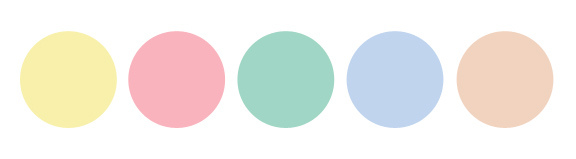
\includegraphics[scale=0.6]{Modelisation/Couleurs/pastels.jpg}
        \caption{Code couleur}
	\label{fig:codecouleur}
\end{figure}
\begin{figure}[hbtp]
    \begin{minipage}[b]{0.4\linewidth}
        \centering 
\includegraphics[scale=0.43]{Modelisation/connexion.png}
        \caption{Fenêtre de connexion}
	\label{fig:connexion}
    \end{minipage}\hfill
    \begin{minipage}[b]{0.48\linewidth}
        \centering 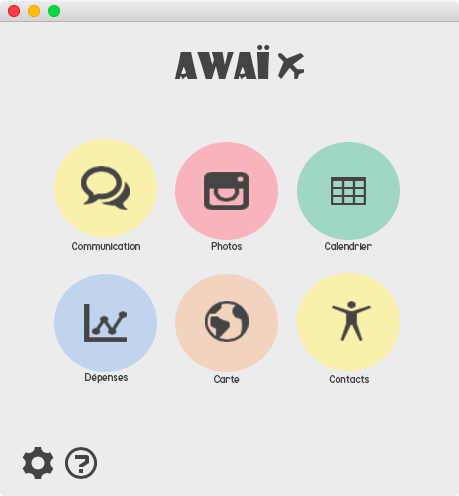
\includegraphics[scale=0.43]{Modelisation/awai.png}
       \caption{Fenêtre principale}
\label{fig:principale}
    \end{minipage}
\end{figure}
\begin{figure}[hbtp]
    \begin{minipage}[b]{0.4\linewidth}
        \centering 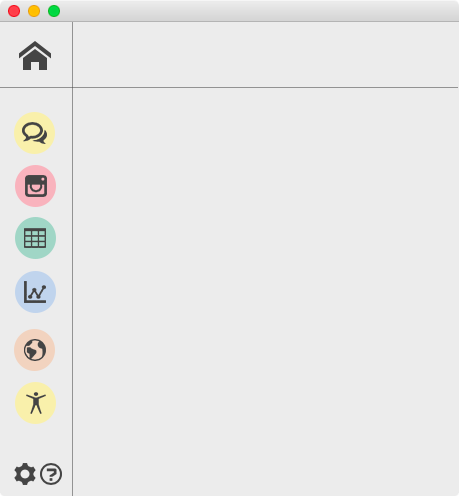
\includegraphics[scale=0.43]{Modelisation/base.png}
        \caption{Base de l'interface}
\label{fig:base}
    \end{minipage}\hfill
    \begin{minipage}[b]{0.48\linewidth}
        \centering 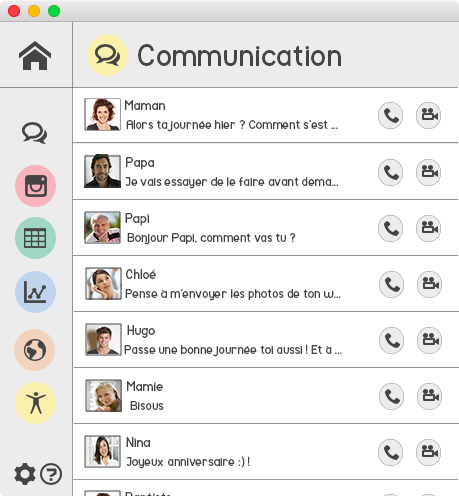
\includegraphics[scale=0.43]{Modelisation/communication.png}
        \caption{Gestion des communications}
        \label{fig:communication}
    \end{minipage}
\end{figure}
\begin{figure}[hbtp]
    \begin{minipage}[b]{0.4\linewidth}
        \centering 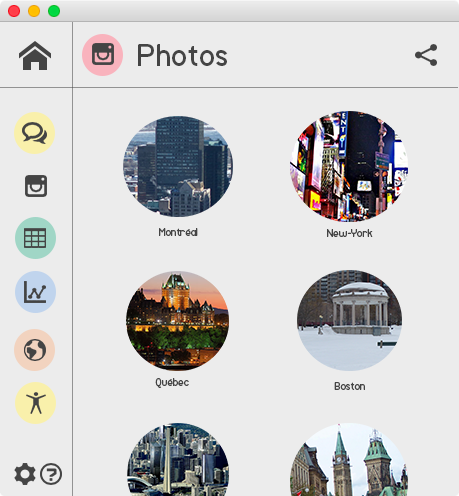
\includegraphics[scale=0.43]{Modelisation/photos.png}
        \caption{Gestion des photos}
                \label{fig:photos}
\label{fig:base}
    \end{minipage}\hfill
    \begin{minipage}[b]{0.48\linewidth}
        \centering 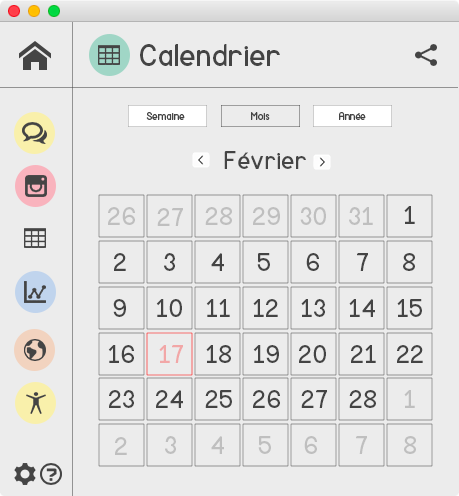
\includegraphics[scale=0.43]{Modelisation/calendrier.png}
        \caption{Gestion du calendrier}
        \label{fig:calendrier1}
    \end{minipage}
\end{figure}
\begin{figure}[hbtp]
    \begin{minipage}[b]{0.4\linewidth}
        \centering 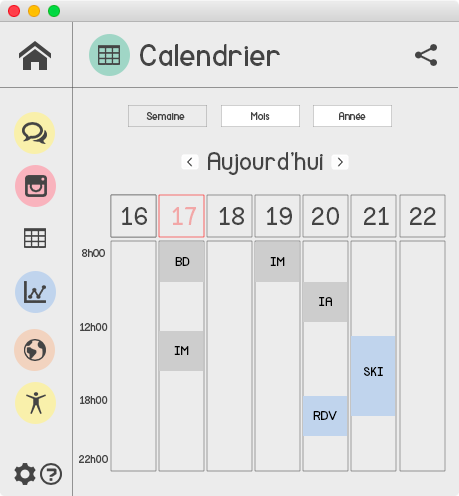
\includegraphics[scale=0.43]{Modelisation/calendrier2.png}
        \caption{Gestion du calendrier}
                \label{fig:calendrier2}
\label{fig:base}
    \end{minipage}\hfill
    \begin{minipage}[b]{0.48\linewidth}
        \centering 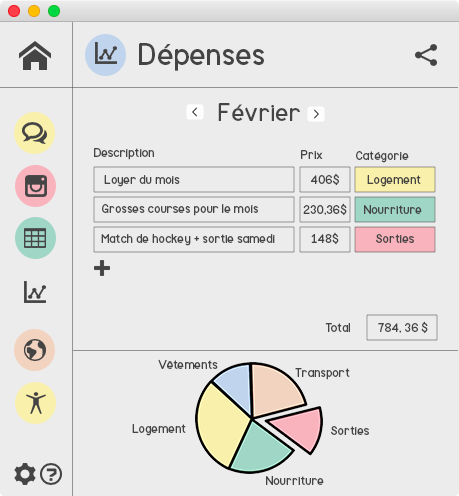
\includegraphics[scale=0.43]{Modelisation/depenses.png}
        \caption{Gestion des dépenses}
         \label{fig:depenses}
    \end{minipage}
\end{figure}
\begin{figure}[hbtp]
    \begin{minipage}[b]{0.4\linewidth}
        \centering 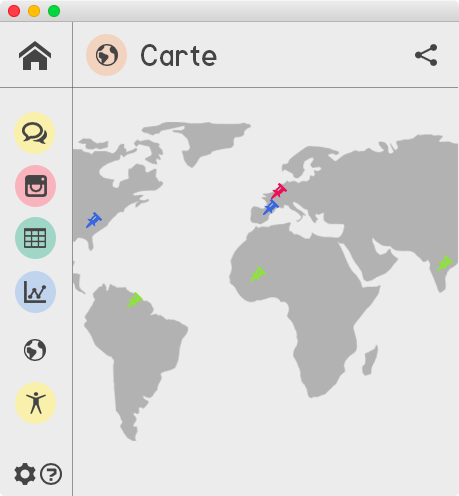
\includegraphics[scale=0.43]{Modelisation/carte.png}
        \caption{Gestion de la carte}
                \label{fig:carte}
\label{fig:base}
    \end{minipage}\hfill
    \begin{minipage}[b]{0.48\linewidth}
        \centering 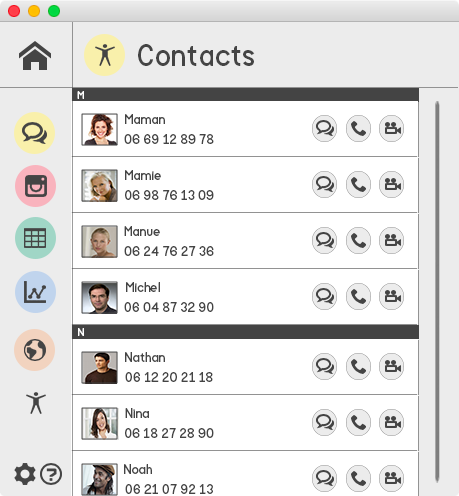
\includegraphics[scale=0.43]{Modelisation/contact.png}
        \caption{Gestion des contacts}
         \label{fig:contact}
    \end{minipage}
\end{figure}


\end{document}